% --------------------------------------------------------------- %
%                       1. TIEKIMO GRANDINĖ                           
% --------------------------------------------------------------- %

\section {Tiekimo grandinė}

Tam, kad būtų galima nagrinėti technologijų taikymą tiekimo grandinėse, reikia suprasti dalykinę sritį, t.y. kokios yra svarbiausios sąvokos, struktūra, vyraujančios problemos ir keliami reikalavimai. Dėl šios priežasties tolimesniuose poskyriuose bus apžvelgiami išvardyti dalykinės srities aspektai.



% --------------------------------------------------------------- %
%                           1.1. SĄVOKA                           
% --------------------------------------------------------------- %

\subsection{Sąvoka}

Tiksliai ir vienareikšmiškai apibrėžti tiekimo grandinę (angl. \textit{Supply chain}) yra ganėtinai sunkus uždavinys. Apskritai, tai yra pakankamai abstrakti sąvoka, kuri kuri laikui bėgant nemažai evoliucionavo ir gali kisti nuo konteksto, kuriame yra naudojama. Pavyzdžiui, grupė akademikų tiekimo grandinę apibrėžė kaip tris arba daugiau šalių, tiesiogiai susijusių su produktų, paslaugų, finansų ir informacijos judėjimo srautais nuo šaltinio iki kliento \cite{mentzer2001defining}. Tuo tarpu Martin Cristopher tiekimo grandinę įvardijo kaip dalyvaujančių organizacijų tinklą, kuris skirtingais procesais ir veiklomis kuria vertę produktų ir paslaugų pavidalu vartotojui \cite{christopher2016logistics}. 

Taip pat Martin Cristopher savo knygoje diskutuoja, kad tiekimo grandinės sąvokoje žodis „tiekimo“ turėtų būti pakeistas žodžiu „paklausos“ (angl. \textit{Demand}), o žodis „grandinė“ žodžiu „tinklas“ (angl. \textit{Network}). Paklausos sąvoka argumentuojama tuo, kad tiekimo grandinė priklauso ne nuo tiekėjų, o nuo rinkos situacijos, t.y paklausos, o žodis „tinklas“ labiau atitiktų struktūrą, kadangi paprastai tiekimo grandinėje dalyvauja daugiau nei vienas tiekėjas ir klientas \cite{christopher2016logistics}. Tokiu būdu tiekimo grandinės modelis (žr. 1 pav.) taptų panašesnis į paklausos tinklo modelį (žr. 2 pav.).

\begin{figure}[H]
    \centering
    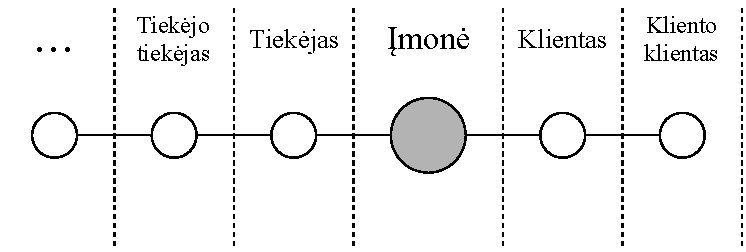
\includegraphics[scale=1]{images/client-supplier-model}
    \caption{Klientų ir tiekėjų sąryšis tiekimo grandinėje}
\end{figure}

Nors tinklo modelis yra arčiau realybės, dėl paprastumo ir platesnio sąvokos žinomumo šiame darbe tiekimo grandinės sąvoka bus naudojama turint galvoje tinklo struktūrą. Taigi, pasinaudoję abiem moksliniais šaltiniais, galime suformuluoti išvestinį tiekimo grandinės apibrėžimą – tai organizacijų, procesų, paslaugų, finansų ir informacijos visuma, dalyvaujanti produkto gyvavimo cikle nuo pradinio tiekėjo iki galutinio kliento.

\begin{figure}[H]
    \centering
    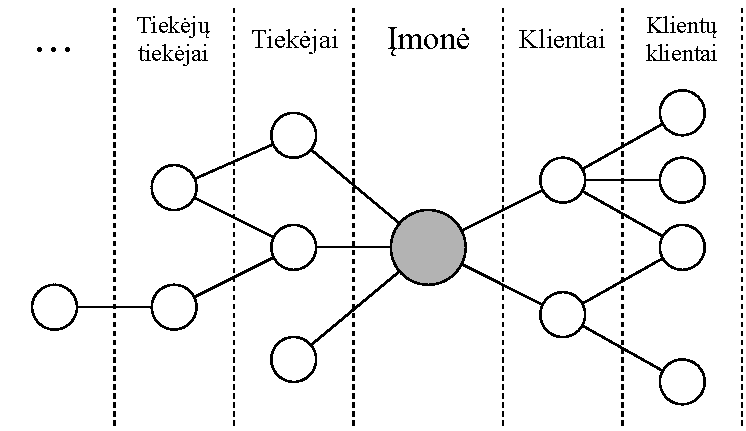
\includegraphics[scale=0.8]{images/demand-network-model}
    \caption{Paklausos tinklo modelis}
\end{figure}

Daugelyje mokslinių straipsnių galime aptikti sąvokas „prieš srovę“ (angl. \textit{Upstream}) ir „pasroviui“ (angl. \textit{Downstream}) \cite{croson2005upstream} \cite{frohlich2001arcs} \cite{vachon2006extending}. Tiekimo grandinės kontekste šie žodžiai reiškia įmonės sąryšį su tiekėjais ir klientais. Pavyzdžiui, viską, kas ateina į įmonę iš tiekėjų, paprastai ateina prieš srovę. Tuo tarpu tai, kas išeina iš įmonės pas klientus, atvirkščiai, pasroviui \cite{christopher2016logistics} (žr. 3 pav.). Prieš srovę ir pasroviui gali judėti ne tik prekės, bet ir pinigai, informacija bei kitos esybės.

\begin{figure}[H]
    \centering
    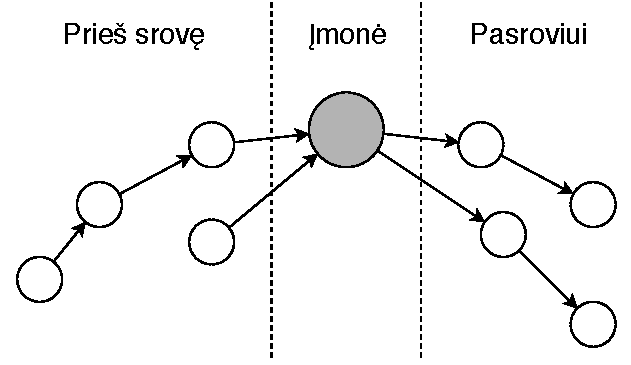
\includegraphics[scale=0.8]{images/supply-chain-upstream-downstream}
    \caption{Įmonės sąryšiai su tiekėjais ir klientais}
\end{figure}



% --------------------------------------------------------------- %
%                          1.2. STRUKTŪRA                           
% --------------------------------------------------------------- %

\subsection{Struktūra}

Nagrinėjant tiekimo grandinės sąvoką ankstesniame skyriuje buvo sužinota, kad yra tiekėjų, klientų ir įmonės rolės. Tačiau tai pernelyg abstraktus modelis, kuris nesuteikia gilesnių žinių apie tiekimo grandinės veikimą. Mums svarbu suprasti kas yra tie tiekėjai ir klientai bei kaip šalys bendrauja tarpusavyje, t.y. kokios veiklos ir procesai vyksta tiekimo grandinėje. 

Tačiau visa tai labai priklauso ir nuo industrijų, kuriose šios tiekimo grandinės funkcionuoja. Pavyzdžiui, procesai ir praktikos, naudojamos maisto pramonėje nebūtinai gali tikti automobilių gamybos industrijoje. Tą patvirtina vien saugumo klausimų skirtumai tarp šių pramonių \cite{marucheck2011product}.

Nagrinėti tikslią realybėje egzistuojančią tiekimo grandinės struktūrą yra sunku ir dėl to, kad įmonės neviešina savo tiekimo grandinės tikslaus gyvavimo ciklo dėl konfidencialumo ir konkurencinių priežasčių. Tačiau moksliniuose ir internetiniuose šaltiniuose galime aptikti nemažai pavyzdinių realybę bandančių atkartoti modelių nuo pat žaliavų surinkimo iki pagaminto produkto pristatymo galutiniam pirkėjui \cite{christopher2016logistics} \cite{webber2009building} \cite{patrick2017continuous} \cite{justin2016customer}. Pasinaudojus jais, autorius sumodeliavo tiekimo grandinės pavyzdinį modelį, aprašytą 3 skyriuje.

Paprastai fizinių produktų tiekimo grandinėje dalyvauja: tiekėjai (angl. \textit{Suppliers}), gamintojai\footnote{Į šią kategoriją įtraukiami pramonininkai, apdirbėjai.} (angl. \textit{Manufacturers}), platintojai (angl. \textit{Distributors}), prekiautojai (angl. \textit{Retailers}) ir galutiniai pirkėjai (angl. \textit{End Customers}) \cite{kopczak2003supply}. Taip pat bet kurioje grandies etape gali dalyvauti išorinės šalys, tokios kaip audito įmonių arba muitų inspektoriai \cite{webber2009building}.

Įvairiuose straipsniuose yra diskutuojama, kad fiziniai produktai keliauja į įmones prieš srovę ir išeina iš įmonės pasroviui, o informacija apie turimus produktus\footnote{Ši informacija naudinga tiekėjams sužinoti apie paklausą \cite{croson2005upstream}.} atvirkščiai – į įmonę patenka pasroviui, o išeina prieš srovę \cite{prajogo2012supply} \cite{croson2005upstream}. Tačiau kyla klausimas, kaip juda informacija apie produktus, finansai ir keliami reikalavimai.

\begin{figure}[H]
    \centering
    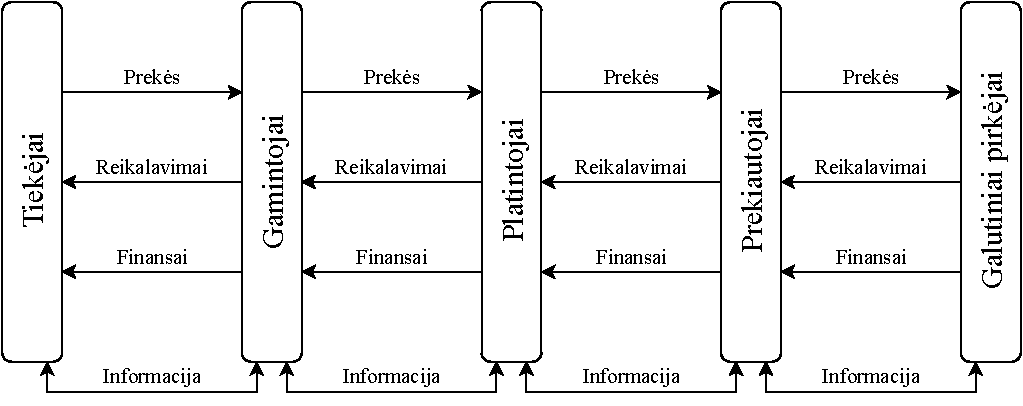
\includegraphics[scale=0.9]{images/supply-chain-entity-flow.pdf}
    \caption{Tiekimo grandinės esybių srautų judėjimas}
\end{figure}

Užsakymus paprastai inicijuoja pasroviui esantys tiekimo grandinės nariai \cite{croson2005upstream}. Tai reiškia, kad finansus ir keliamus reikalavimus teikia taip pat pasroviui esantys grandinės nariai. Tuo tarpu detali informacija apie produktus ir jų kokybę į įmones patenka prieš srovę. Tai gali būti socialiai atsakinga informacija\footnote{Šios informacijos poreikis kyla iš keliamų reikalavimų.}, susijusi su aplinkosauga, darbuotojų darbo sąlygomis, cheminių produktų naudojimu ar inspektorių vertinimais \cite{mani2015supply} \cite{vachon2006extending}. Tai gali būti ir verslo informacija apie esamą prekių kiekį, lokaciją, kokybę ir t.t. 4 paveikslėlis vaizduoja įvairių esybių judėjimą tarp šiame poskyryje išvardytų tiekimo grandinės narių.



% --------------------------------------------------------------- %
%                   1.3. ŠIANDIENINĖS PROBLEMOS                           
% --------------------------------------------------------------- %

\subsection{Šiandieninės problemos}

Natūralu, kad įmonėms, dalyvaujančioms tiekimo grandinėse, tenka kažkokiu būdu suvaldyti visus esybių srautus. Tam į pagalbą ateina IT sprendimai, kurių vienas – verslo valdymo sistemos (angl. \textit{Enterprise Resource Planning}), toliau – ERP. Tai yra programinė įranga, kuri bando apjungti visus įmonės duomenis ir procesus, arba paprasčiau – duomenų bazė, kurioje gali būti laikomi įvairūs duomenys \cite{ozcan2016software}. 

ERP turi savo privalumų. Sistemos leidžia matyti bendrą verslo vaizdą suteikdamos duomenų bazę su visomis transakcijomis, kurias galima įrašyti, stebėti, apdoroti ir pranešti \cite{neubert2018collaboration}. Taip yra pasiekiamas pagrindinis tikslas – centralizuotas įmonės valdymas \cite{ozcan2016software}. Tačiau dalis įmonių vis dėlto nesirenka ERP dėl aukštos sistemų kainos, ilgo adaptacijos laikotarpio ir įmonės vidinių technologinės infrastruktūros nepajėgumų \cite{ozcan2016software}. Dar viena svari priežastis – tradicinės ERP sistemos neleidžia stebėti individualių produktų \cite{garg2018supply}. 

Ir tai tik programinės įrangos pavyzdys. Tiekimo grandinės apimtis yra plati, todėl visose jos grandyse kyla skirtingos problemos. Pavyzdžiai: gendantys produktai dėl prastovų \cite{briano2010resiliency}, pasimetantys dokumentai ir kroviniai \cite{huber2007vendor}, socialinės ir gamtosaugos problemos \cite{mani2015supply} \cite{vachon2006extending}, produktų padirbinėjimai \cite{huber2007vendor} ir dar daug kitų. Šios problemos indikuoja, kad yra poreikis IT technologijoms, kurios užtiktų jų prevenciją. Potenciali dalį problemų išspręsti siekianti technologija bus apžvelgiama kitame skyriuje.